\subsection*{Senyal del far}
\addcontentsline{toc}{subsection}{Senyal del far}


La comunicació mitjançant llum visible té una llarga història, encara que la tecnologia VLC basada en LED es va inventar al segle XXI. La història prèvia de VLC es va basar en l'ús de llum solar, foc o diferents tipus de làmpades per transmetre informació. Per exemple, la llum del sol es reflectia als miralls, el foc s'usava als fars, encara que aquest foc ha estat sistituït per llums com s'apareixia a la figura següent; i en la comunicació directa de codi Morse.


\begin{figure}[h!]
    \centering
    \includegraphics[width=80mm]{comunicacióLlum.png}
    \caption{Comunicació a través del llum}
\end{figure}


\subsection*{1841: Descubriment de Reflexió total}
\addcontentsline{toc}{subsection}{1841: Descubriment de Reflexió total}

La reflexió total és el fenomen físic que es produeix quan un raig de llum incideix amb un angle superior a l'angle crític en una superfície transparent d'índex de refracció alt. Per angles d'incidència majors o iguals a l'angle crític, tota l'energia és reflectida cap al medi incident.
S'utilitza en la fibra òptica, fent que l'índex de refracció de l'interior sigui més gran que l'aire. D'aquesta manera un raig que emetem des del principi no surt del fil fins que no es talla. Es pot utilitzar per les telecomunicacions o per la cirurgia.

\begin{figure}[h!]
    \centering
    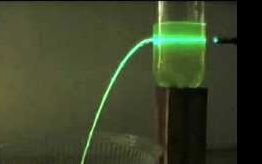
\includegraphics[width=80mm]{refluxiototal.png}
    \caption{Teoría reflexió total}
\end{figure}


\subsection*{1880: Bell va patentar el fotòfon}
\addcontentsline{toc}{subsection}{1880: Bell va patentar el fotòfon}

El primer equip sofisticat de comunicació sense fils va ser el fotòfon, inventat per Alexander Grahan Bell l'any 1880.
El fotòfon permetia la transmissió de so mitjançant una emissió de llum, va ser similar al telèfon, l'única diferencia evident va ser que aquest va utilitzar la llum com a mitjà per a fer l'intercanvi d'informació, i el telèfon va confiar en l'electricitat.

\begin{figure}[h!]
    \centering
    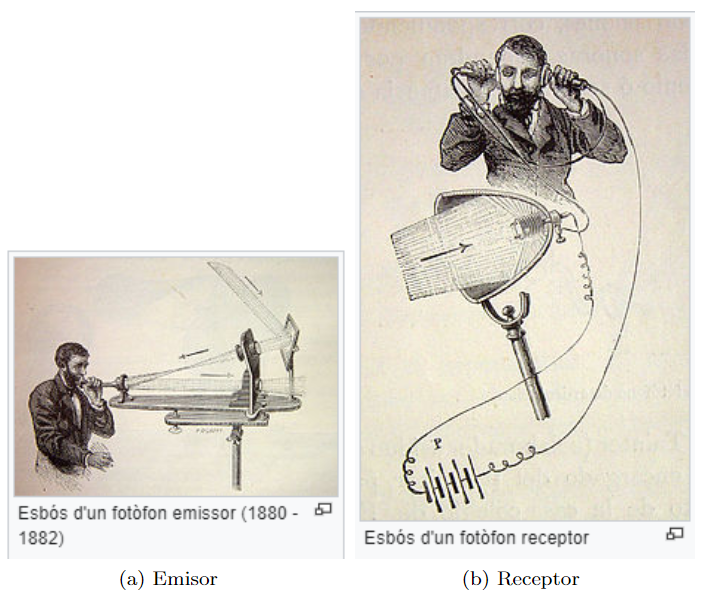
\includegraphics[width=80mm]{fotofon.png}
    \caption{Fotofòn}
\end{figure}


\subsection*{1887: }
\addcontentsline{toc}{subsection}{Altres treballs}

\begin{itemize}
    \item El 2003 al Laboratori Nakagawa, a la Universitat de Keio, Japó, utilitzant LED per transmetre dades mitjançant la llum visible. Des de llavors hi ha hagut nombroses activitats de recerca centrades en VLC.
    \item El 2006, investigadors del CICTR de Penn State van proposar una combinació de comunicació de línia elèctrica (PLC) i LED de llum blanca per proporcionar accés de banda ampla per a aplicacions interiors. Aquesta investigació va suggerir que VLC es podria desplegar com una solució perfecta d'última milla en el futur.
    \item El gener de 2010, un equip d'investigadors de Siemens i Fraunhofer Institute for Telecommunications, Heinrich Hertz Institute, a Berlín, va demostrar la transmissió a 500 Mbit/s amb un LED blanc a una distància de 5 metres (16 peus) i 100 Mbit/s més. distància més llarga utilitzant cinc LED.
    \item El procés d'estandardització de VLC es realitza dins del grup de treball IEEE 802.15.7.
    \item El desembre de 2010, St. Cloud, Minnesota, va signar un contracte amb LVX Minnesota i es va convertir en el primer a desplegar comercialment aquesta tecnologia.

\end{itemize}


\subsection*{Primer LED Li-Fi}
\addcontentsline{toc}{subsection}{Primer LED Li-Fi}

La tecnologia Li-Fi va ser proposada per primera vegada pel professor Harald Haas de la Universitat d'Edimburg durant una conferència TED Talk al juliol de 2011. En aquesta presentació, el professor Haas va descriure la possibilitat d'utilitzar la llum LED per a transmetre dades de manera inalàmbrica, una idea que va conduir al desenvolupament de la tecnologia Li-Fi.

Els sistemes de posicionament interior basats en VLC s'han convertit en un tema atractiu. La investigació d'ABI preveu que podria ser una solució clau per desbloquejar el "mercat d'ubicació interior" de 5.000 milions de dòlars. Les publicacions han estat provinents del laboratori Nakagawa, ByteLight va presentar una patent sobre un sistema de posicionament de llum que utilitzava el reconeixement de polsos digitals LED el març de 2012. COWA a Penn State i altres investigadors d'arreu del món.


\subsection*{Altres treball recents}
\addcontentsline{toc}{subsection}{Altres treballs recents}


\begin{itemize}
    \item Una altra aplicació és en el món de les joguines, gràcies a la implementació rendible i de baixa complexitat, que només requereix un microcontrolador i un LED com a frontal òptic.
    \item Els VLC es poden utilitzar per proporcionar seguretat. Són especialment útils en xarxes de sensors corporals i xarxes d'àrea personal.
    \item L'octubre de 2014, Axrtek va llançar un sistema comercial bidireccional RGB LED VLC anomenat MOMO que transmet cap avall i cap amunt a velocitats de 300 Mbit/s i amb un abast de 25 peus.
    \item El maig de 2015, Philips va col·laborar amb l'empresa de supermercats Carrefour per oferir serveis basats en la localització de VLC als telèfons intel·ligents dels compradors en un hipermercat de Lille, França. El juny de 2015, dues empreses xineses, Kuang-Chi i Ping An Bank, es van associar per introduir una targeta de pagament que comunica informació mitjançant una llum visible única. El març de 2017, Philips va establir els primers serveis basats en la ubicació VLC per als telèfons intel·ligents dels compradors a Alemanya. La instal·lació es va presentar a l'EuroShop de Düsseldorf (5-9 de març). Com a primer supermercat a Alemanya, un supermercat Edeka a Düsseldorf-Bilk està utilitzant el sistema, que ofereix una precisió de posicionament de 30 centímetres que es pot aconseguir, que compleix les demandes especials de la venda al detall d'aliments. Els sistemes de posicionament interior basats en VLCes poden utilitzar en llocs com hospitals, residències de gent gran, magatzems i oficines grans i obertes per localitzar persones i controlar vehicles robòtics interiors.
\end{itemize}